\documentclass[a4paper]{article}
\usepackage{iftex}
\ifPDFTeX
  \usepackage{vntex}
\else
  % XeLaTeX / LuaLaTeX (vi du Overleaf chon compiler khac): dung fontspec
  \usepackage{fontspec}
  \setmainfont{TeX Gyre Termes}
  \setsansfont{TeX Gyre Heros}
  \setmonofont{TeX Gyre Cursor}
\fi
%\usepackage[english,vietnam]{babel}
%\usepackage[utf8]{inputenc}

%\usepackage[utf8]{inputenc}
%\usepackage[francais]{babel}
\usepackage{a4wide,amssymb,epsfig,latexsym,multicol,array,hhline,fancyhdr}
\usepackage{booktabs}
\usepackage{amsmath}
\usepackage{lastpage}
\usepackage[lined,boxed,commentsnumbered]{algorithm2e}
\usepackage{enumerate}
\usepackage{color}
\usepackage{graphicx}							% Standard graphics package
\usepackage{array}
\usepackage{tabularx, caption}
\usepackage{multirow}
\usepackage[framemethod=tikz]{mdframed}% For highlighting paragraph backgrounds
\usepackage{multicol}
\usepackage{rotating}
\usepackage{graphics}
\usepackage{geometry}
\usepackage{setspace}
\usepackage{epsfig}
\usepackage{tikz}
\usepackage{listings}
\usetikzlibrary{arrows,snakes,backgrounds}
\usepackage{hyperref}
\hypersetup{urlcolor=blue,linkcolor=black,citecolor=black,colorlinks=true} 
%\usepackage{pstcol} 								% PSTricks with the standard color package

\newtheorem{theorem}{{\bf Định lý}}
\newtheorem{property}{{\bf Tính chất}}
\newtheorem{proposition}{{\bf Mệnh đề}}
\newtheorem{corollary}[proposition]{{\bf Hệ quả}}
\newtheorem{lemma}[proposition]{{\bf Bổ đề}}

\everymath{\color{blue}}
%\usepackage{fancyhdr}
\setlength{\headheight}{40pt}
\pagestyle{fancy}
\fancyhead{} % clear all header fields
\fancyhead[L]{
 \begin{tabular}{rl}
    \begin{picture}(25,15)(0,0)
    \put(0,-8){
\includegraphics[width=8mm, height=8mm]{logoITSGUsmall.png}}
    %\put(0,-8){\epsfig{width=10mm,figure=hcmut.eps}}
   \end{picture}&
	%\includegraphics[width=8mm, height=8mm]{hcmut.png} & %
	\begin{tabular}{l}
		\textbf{\bf \ttfamily Trường Đại học Sài Gòn}\\
		\textbf{\bf \ttfamily Khoa Công Nghệ Thông Tin}
	\end{tabular} 	
 \end{tabular}
}
\fancyhead[R]{
	\begin{tabular}{l}
		\tiny \bf \\
		\tiny \bf 
	\end{tabular}  }
\fancyfoot{} % clear all footer fields
\fancyfoot[L]{\scriptsize \ttfamily Bài tập lớn 1 (giữa kì) môn Công nghệ phần mềm - Năm học 2026-2027}
\fancyfoot[R]{\scriptsize \ttfamily Trang {\thepage}/\pageref{LastPage}}
\renewcommand{\headrulewidth}{0.3pt}
\renewcommand{\footrulewidth}{0.3pt}


%%%
\setcounter{secnumdepth}{4}
\setcounter{tocdepth}{3}
\makeatletter
\newcounter {subsubsubsection}[subsubsection]
\renewcommand\thesubsubsubsection{\thesubsubsection .\@alph\c@subsubsubsection}
\newcommand\subsubsubsection{\@startsection{subsubsubsection}{4}{\z@}%
                                     {-3.25ex\@plus -1ex \@minus -.2ex}%
                                     {1.5ex \@plus .2ex}%
                                     {\normalfont\normalsize\bfseries}}
\newcommand*\l@subsubsubsection{\@dottedtocline{3}{10.0em}{4.1em}}
\newcommand*{\subsubsubsectionmark}[1]{}
\makeatother

\definecolor{dkgreen}{rgb}{0,0.6,0}
\definecolor{gray}{rgb}{0.5,0.5,0.5}
\definecolor{mauve}{rgb}{0.58,0,0.82}

\lstset{frame=tb,
	language=Matlab,
	aboveskip=3mm,
	belowskip=3mm,
	showstringspaces=false,
	columns=flexible,
	basicstyle={\small\ttfamily},
	numbers=none,
	numberstyle=\tiny\color{gray},
	keywordstyle=\color{blue},
	commentstyle=\color{dkgreen},
	stringstyle=\color{mauve},
	breaklines=true,
	breakatwhitespace=true,
	tabsize=3,
	numbers=left,
	stepnumber=1,
	numbersep=1pt,    
	firstnumber=1,
	numberfirstline=true
}

\newcommand{\fillme}[1]{{\color{red}[#1]}}
\begin{document}

\begin{titlepage}
\begin{center}
TRƯỜNG ĐẠI HỌC SÀI GÒN \\
KHOA CÔNG NGHỆ THÔNG TIN
\end{center}
\vspace{1cm}

\begin{figure}[h!]
\begin{center}

\includegraphics[width=3cm]{logoITSGU.png}
\end{center}
\end{figure}

\vspace{1cm}

\begin{center}
\begin{tabular}{c}
	\multicolumn{1}{l}{\textbf{{\Large CÔNG NGHỆ PHẦN MỀM}}}\\
	~~\\
	\hline
	\\
	\multicolumn{1}{l}{\textbf{{\large Bài tập lớn 1 (giữa kì): xây dựng ứng dụng theo Agile Scrum}}}\\
	\\
	\textbf{{\huge BrewLite -- Ứng dụng đặt đồ uống}}\\
	\\
	\hline
\end{tabular}
\end{center}

\vspace{3cm}

\begin{table}[h]
\begin{tabular}{rrl}
\hspace{5 cm} & GVHD: &Từ Lăng Phiêu\\
& SV: & Nguyễn Lê Nhựt Thắng - 3124560085\\
& & Hồ Thiên Ngân - 3124410224 \\
& & Hà Thiên Long - 3124410193 \\
& & Giản Thiên Lực - 3124410206\\
\end{tabular}
\vspace{1.5 cm}
\end{table}

\begin{center}
{\footnotesize TP. HỒ CHÍ MINH, THÁNG 11/2026}
\end{center}
\end{titlepage}

\thispagestyle{empty}

\newpage
\tableofcontents
\newpage

%%%%%%%%%%%%%%%%%%%%%%%%%%%%%%%%%
\section{Phần giới thiệu}
\subsection{Bối cảnh và mục tiêu}
BrewLite là ứng dụng web mobile-first giúp khách đặt đồ uống và thanh toán không dùng tiền mặt: xem thực đơn, chọn size, mức đường, mức đá và topping, thêm vào giỏ, đăng nhập, đặt đơn, xem tổng tiền sau khuyến mãi, thanh toán mô phỏng (Ví/Thẻ), xem xác nhận và lịch sử đơn. Bài tập lớn gồm 10 task theo Agile Scrum (mỗi task 1 điểm), kèm bốn nghiệp vụ backend nâng cao ở Task 10. Hạn nộp: 15/11/2026.

\subsection{Công nghệ và sản phẩm bàn giao}
\begin{center}
\small\everymath{}
\begin{tabular}{@{}p{2.8cm}p{11.2cm}@{}}
\toprule
\textbf{Lớp} & \textbf{Công nghệ / liên kết} \\ \midrule
Frontend & Next.js (mobile-first): thực đơn, chi tiết món, giỏ hàng (React Context, localStorage), thanh toán hai bước, xác nhận và lịch sử đơn; thanh tab ở đáy màn hình trên điện thoại \\
Backend & NestJS, class-validator, JWT, bcrypt \\
Cơ sở dữ liệu & PostgreSQL 16, Prisma 7 (migration, seed); 9 bảng, ERD ở Hình~\ref{fig:erd} (phụ lục) \\
Kiểm thử, vận hành & Vitest, Supertest (PostgreSQL thật); Postman/newman; Docker Compose \\
Mã nguồn & \url{https://github.com/tthan-prog/BrewLite-AS1}, nhánh \texttt{main} \\
Bản chạy & Chạy cục bộ bằng \texttt{docker compose up --build} (frontend cổng 3000, backend 3001, PostgreSQL 5432), hướng dẫn trong \texttt{README.md} \\ \bottomrule
\end{tabular}
\end{center}

%%%%%%%%%%%%%%%%%%%%%%%%%%%%%%%%%
\subsection{Product Vision, yêu cầu và user story}
\textit{Product Vision:} ``BrewLite giúp khách hàng đặt và thanh toán đồ uống \textbf{không dùng tiền mặt} chỉ trong vài chạm, giảm thời gian xếp hàng và nhận đơn nhanh tại quầy.'' \textbf{Bên liên quan:} khách hàng; barista (ngoài phạm vi MVP, chỉ có API cho STAFF); Product Owner (Hà Thiên Long, tạm); giảng viên; nhóm phát triển; đơn vị thanh toán (mô phỏng).

\textbf{Chức năng:} (1) menu kèm hình, tên, giá; (2) chi tiết, chọn size và topping; (3) giỏ hàng thêm/sửa/xóa, tự tính tổng tiền; (4) đăng ký, đăng nhập bằng JWT; (5) tạo đơn và thanh toán không tiền mặt; (6) xác nhận đơn và lịch sử đơn. \textbf{Phi chức năng:} API phản hồi dưới 500\,ms với dữ liệu mẫu; mật khẩu băm, JWT, validate đầu vào; phù hợp trên các trình duyệt web.

\begin{mdframed}[hidealllines=true,backgroundcolor=green!8]
\small\textbf{US-05 -- Thanh toán không tiền mặt.} Là một khách hàng, tôi muốn thanh toán bằng ví điện tử hoặc thẻ để không cần mang tiền mặt. \textit{Tiêu chí chấp nhận:} khi giỏ có sản phẩm, nút ``Thanh toán'' hiển thị tổng tiền; chọn Ví hoặc Thẻ rồi xác nhận thì đơn thành PAID; nếu lỗi, đơn ở PAYMENT\_FAILED và giỏ hàng được giữ; thành công thì hiển thị mã đơn. \textit{Quyết định của nhóm:} Task 6 tạo đơn PENDING, Task 8 chuyển PAID hoặc PAYMENT\_FAILED.
\end{mdframed}

%%%%%%%%%%%%%%%%%%%%%%%%%%%%%%%%%
\section{Quy trình Scrum và phân công}
\subsection{Vai trò và phân công thành viên}
Nhóm gồm 4 thành viên; vai trò là người chịu trách nhiệm chính của từng task (theo thỏa thuận nhóm). Daily Scrum 20:00, tối đa 15 phút; mỗi thành viên một nhánh riêng, gộp vào \texttt{main} qua Pull Request.
\begin{center}
\small\everymath{}
\begin{tabular}{@{}p{3.7cm}p{3.7cm}p{6.2cm}@{}}
\toprule
\textbf{Thành viên} & \textbf{Vai trò} & \textbf{Task phụ trách} \\ \midrule
Nguyễn Lê Nhựt Thắng (A) & Scrum Master, backend & 1; backend task 2, 7, 8, 9, 10 \\
Hồ Thiên Ngân (B) & Backend: dữ liệu, đơn hàng & 2 (schema, seed), 6, 10 \\
Hà Thiên Long (C) & Frontend, kiểm thử, PO tạm & giao diện 7, 9; Product Vision, FR/NFR \\
Giản Thiên Lực (D) & Frontend & 3, 4, 5 \\
\bottomrule
\end{tabular}
\end{center}

\subsection{Ba Sprint}
\begin{center}
\small\everymath{}
\begin{tabular}{@{}p{1.4cm}p{2.0cm}p{3.0cm}p{1.2cm}p{1.5cm}p{3.2cm}@{}}
\toprule
\textbf{Sprint} & \textbf{Thời gian} & \textbf{Cam kết (điểm)} & \textbf{Xong} & \textbf{Còn lại} & \textbf{Ghi chú} \\ \midrule
1 & 14--18/10 & 11 & 2 & 9 & Trễ, chỉ xong Task 1 \\
2 & 19--22/10 & 22 (13 mới + 9 tồn) & 14 & 8 & Còn Task 7 backend \\
3 & 23--25/10 & 24 (16 mới + 8 tồn) & 24 & 0 & Đủ 10 task, đạt DoD \\
Hoàn thiện & 26/10--13/11 & -- & -- & -- & Thử lại luồng như khách hàng, hoàn thiện giao diện, báo cáo \\
\bottomrule
\end{tabular}
\end{center}
Mỗi task chỉ tính hoàn thành khi đạt Definition of Done: chạy được và không lỗi build; commit rõ ràng, PR được người khác xem; API validate và giao diện có loading, lỗi; README có hướng dẫn chạy. Điểm ước lượng (do Product Owner tạm) tổng 40 điểm; burndown ở Hình~\ref{fig:burndown} (phụ lục).

%%%%%%%%%%%%%%%%%%%%%%%%%%%%%%%%%
%%%%%%%%%%%%%%%%%%%%%%%%%%%%%%%%%
\section{Kết quả thực hiện 10 task}
\subsection{Tổng hợp theo task}
\begin{center}
\small\everymath{}\raggedright
\begin{tabular}{@{}p{0.8cm}p{3.0cm}p{3.0cm}p{1.7cm}p{4.5cm}@{}}
\toprule
\textbf{Task} & \textbf{Nội dung} & \textbf{Phụ trách} & \textbf{Nghiệm thu} & \textbf{Kết quả} \\ \midrule
1 & Khởi tạo dự án & A & B & Monorepo, README, \texttt{/health} \\
2 & API sản phẩm & A (B: schema) & D & \texttt{GET /products}, 12 sản phẩm mẫu \\
3 & Trang Menu & D & A & Gọi API, loading, rỗng, lỗi \\
4 & Chi tiết, size, topping & D & A & Size S/M/L, phụ phí +0/+5.000/+10.000đ \\
5 & Giỏ hàng & D & A & Thêm, sửa, xóa, tổng tiền, số món; lưu bằng React Context và localStorage \\
6 & API tạo đơn & B & A & \texttt{POST /orders} (JWT, validate, PENDING, mức đường/đá) \\
7 & Đăng ký, đăng nhập & A; C (giao diện) & B & bcrypt, JWT, guard, trang đăng nhập/đăng ký \\
8 & Thanh toán & A; D (giao diện) & C & Đặt đơn rồi thanh toán; \texttt{POST /payments}, thử lại khi lỗi \\
9 & Xác nhận, lịch sử, bàn giao & C; A (API) & A & \texttt{/orders/me}, xác nhận có từng món, Docker \\
10 & Nghiệp vụ backend & A, B & A, C & Bốn nghiệp vụ và ba test bắt buộc (mục 3.2) \\
\bottomrule
\end{tabular}
\end{center}

\subsection{Task 10 -- nghiệp vụ backend}
Bốn nghiệp vụ: (1) máy trạng thái đơn (PENDING, PAID, PREPARING, READY, COMPLETED, thêm PAYMENT\_FAILED và CANCELLED), mọi chuyển trạng thái đi qua một hàm kiểm tra duy nhất; (2) thanh toán idempotent bằng \texttt{Idempotency-Key}, ràng buộc duy nhất theo \texttt{(userId, key)}; (3) kiểm soát tồn kho đồng thời bằng cập nhật có điều kiện \texttt{UPDATE ... WHERE stock >= n} trong transaction khi tạo đơn, một dạng khóa lạc quan (optimistic) không cần cột \texttt{version}: không bán quá số lượng, hủy đơn thì hoàn kho; tồn kho tính theo từng sản phẩm, mỗi món tối đa 50 ly, mỗi đơn tối đa 50 dòng món; (4) mã khuyến mãi (\texttt{WELCOME10} giảm 10\%) và điểm thưởng (1 điểm cho mỗi 10.000 đồng, cộng khi đơn PAID).


\begin{figure}[h!]
\centering
\resizebox{\textwidth}{!}{%
\begin{tikzpicture}[>=latex,
  every node/.style={font=\scriptsize\ttfamily},
  st/.style={draw,rounded corners,fill=gray!8,minimum width=2.4cm,minimum height=0.7cm},
  ok/.style={st,fill=green!15}, bad/.style={st,fill=red!10}, fin/.style={st,fill=gray!25},
  lb/.style={font=\tiny\rmfamily}]
\node[st]  (p) at (0,0) {PENDING};
\node[st]  (a) at (4,0) {PAID};
\node[st]  (r) at (8,0) {PREPARING};
\node[st]  (y) at (12,0) {READY};
\node[ok]  (c) at (16,0) {COMPLETED};
\node[bad] (f) at (0,-2.2) {PAYMENT\_FAILED};
\node[fin] (x) at (6,-2.2) {CANCELLED};
\draw[->] (p) -- node[above,lb]{thanh toán OK} (a);
\draw[->] (a) -- node[above,lb]{nhân viên nhận} (r);
\draw[->] (r) -- node[above,lb]{pha xong} (y);
\draw[->] (y) -- node[above,lb]{giao khách} (c);
\draw[->] ([xshift=-0.5cm]p.south) -- node[left,lb]{lỗi} ([xshift=-0.5cm]f.north);
\draw[->] ([xshift=0.5cm]f.north) -- node[right,lb]{thử lại} ([xshift=0.5cm]p.south);
\draw[->] (p.south east) -- node[above,sloped,lb]{hủy} (x.north west);
\draw[->] (f) -- node[above,lb]{hủy} (x);
\draw[->] (a.south) -- node[right,lb]{hủy} (x.north east);
\end{tikzpicture}}
\caption{Máy trạng thái đơn hàng. Bảng \texttt{ORDER\_TRANSITIONS} trong \texttt{order-state.ts}; mọi chuyển trạng thái không có mũi tên bị \texttt{assertTransition} từ chối (HTTP 400).}
\end{figure}


%%%%%%%%%%%%%%%%%%%%%%%%%%%%%%%%%
\section{Kết quả kiểm thử}
\subsection{Số lượng và kết quả test}
\begin{center}
\small\everymath{}
\begin{tabular}{@{}p{4.2cm}p{2.2cm}p{1.8cm}p{5.0cm}@{}}
\toprule
\textbf{Mức} & \textbf{Công cụ} & \textbf{Số test} & \textbf{Kết quả} \\ \midrule
Unit & Vitest & 22 & 22/22 đạt \\
Tích hợp (PostgreSQL thật) & Vitest + Supertest & 33 & 33/33 đạt \\
Kiểm thử API trên hệ thống đang chạy & Postman/newman & 51 request & 85/85 kiểm tra đạt \\
\bottomrule
\end{tabular}
\end{center}
Chạy ngày 13/11/2026 bằng \texttt{npm test} và \texttt{npm run test:e2e} trong thư mục \texttt{backend}, CSDL PostgreSQL chạy bằng Docker Compose (ảnh kết quả: Hình~\ref{fig:testunit} và~\ref{fig:teste2e}, phụ lục). Test tích hợp gửi yêu cầu HTTP thật vào ứng dụng NestJS, kiểm tra từng API, phân quyền, validate, giá theo size/topping, mức đường/đá, khuyến mãi, điểm thưởng và ba test bắt buộc của Task 10. Bộ Postman (\texttt{docs/postman}, kịch bản ở \texttt{docs/kich-ban-test-backend.md}) gọi API trên hệ thống chạy bằng Docker, xếp theo Task 1--10, gồm cả các trường hợp lỗi (thiếu token, dữ liệu sai, mã khuyến mãi sai, chuyển trạng thái sai).

\subsection{Ba test bắt buộc của Task 10}
\begin{itemize}\setlength{\itemsep}{0pt}\setlength{\parskip}{0pt}
    \item (a) Chặn chuyển trạng thái sai: đơn PAID không nhảy thẳng sang COMPLETED (HTTP 400) -- \textbf{đạt}.
    \item (b) Gửi hai lần cùng \texttt{Idempotency-Key} chỉ tạo một đơn và không thanh toán lần hai -- \textbf{đạt}.
    \item (c) 20 yêu cầu đặt đồng thời khi kho còn 5: đúng 5 đơn thành công, không âm kho -- \textbf{đạt}.
\end{itemize}

%%%%%%%%%%%%%%%%%%%%%%%%%%%%%%%%%
\section{Bàn giao và nhìn lại}
\textbf{Bàn giao:} mã nguồn trên Git; \texttt{docker compose up --build} chạy đủ db, backend, frontend; README hướng dẫn cài đặt, chạy, kiểm thử; demo luồng thực đơn, giỏ hàng, đăng nhập, đặt đơn với mã khuyến mãi, thanh toán lỗi rồi thử lại, xác nhận, lịch sử, cả trên giao diện điện thoại.

\textbf{Retrospective.} Làm tốt: theo đường găng và có test chứng minh nghiệp vụ Task 10; README và Docker giúp chạy lại dễ. Cần cải thiện: bắt đầu muộn (Sprint 1 trễ 9 điểm); phân bố commit giữa các thành viên chưa đều (không tính commit gộp nhánh: A 30, B 4, C 1, D 1 trên 36 commit; A tích hợp phần lớn mã); giai đoạn hoàn thiện cho thấy cần tự thử luồng như khách hàng sớm hơn, ngay trong từng Sprint; nghiệm thu chéo mới ghi trong tài liệu nhóm, chưa có Approve trên từng Pull Request.

%%%%%%%%%%%%%%%%%%%%%%%%%%%%%%%%%
\textbf{Backlog sau:} giao diện barista; cổng thanh toán thật; cho khách tự hủy đơn chưa thanh toán.

{\small
\begin{thebibliography}{80}

\bibitem{scrum}
Ken Schwaber, Jeff Sutherland,
``\textbf{The Scrum Guide}'',
\textit{link: https://scrumguides.org/scrum-guide.html}, 2020, lần truy cập cuối: 26/10/2026.

\bibitem{de}
Khoa CNTT, Trường Đại học Sài Gòn, ``\textbf{Bài tập lớn BrewLite (VER 1.0)}'', \textit{môn Công nghệ phần mềm, học kỳ I năm học 2026--2027}.

\bibitem{docs}
Tài liệu chính thức: NestJS (docs.nestjs.com), Next.js (nextjs.org/docs), Prisma (prisma.io/docs).

\end{thebibliography}}

\clearpage
\appendix
\section{Ảnh minh họa luồng chính}
Ảnh chụp ngày 13/11/2026 từ nhánh \texttt{main} chạy cục bộ bằng Docker Compose, dữ liệu mẫu từ seed, tài khoản \texttt{customer@brewlite.com}. Mã đơn là 34 vì các lần chạy test trước đó đã dùng các mã nhỏ hơn (PostgreSQL không đặt lại bộ đếm khóa chính khi xóa dữ liệu).

\begin{figure}[h!]
\centering
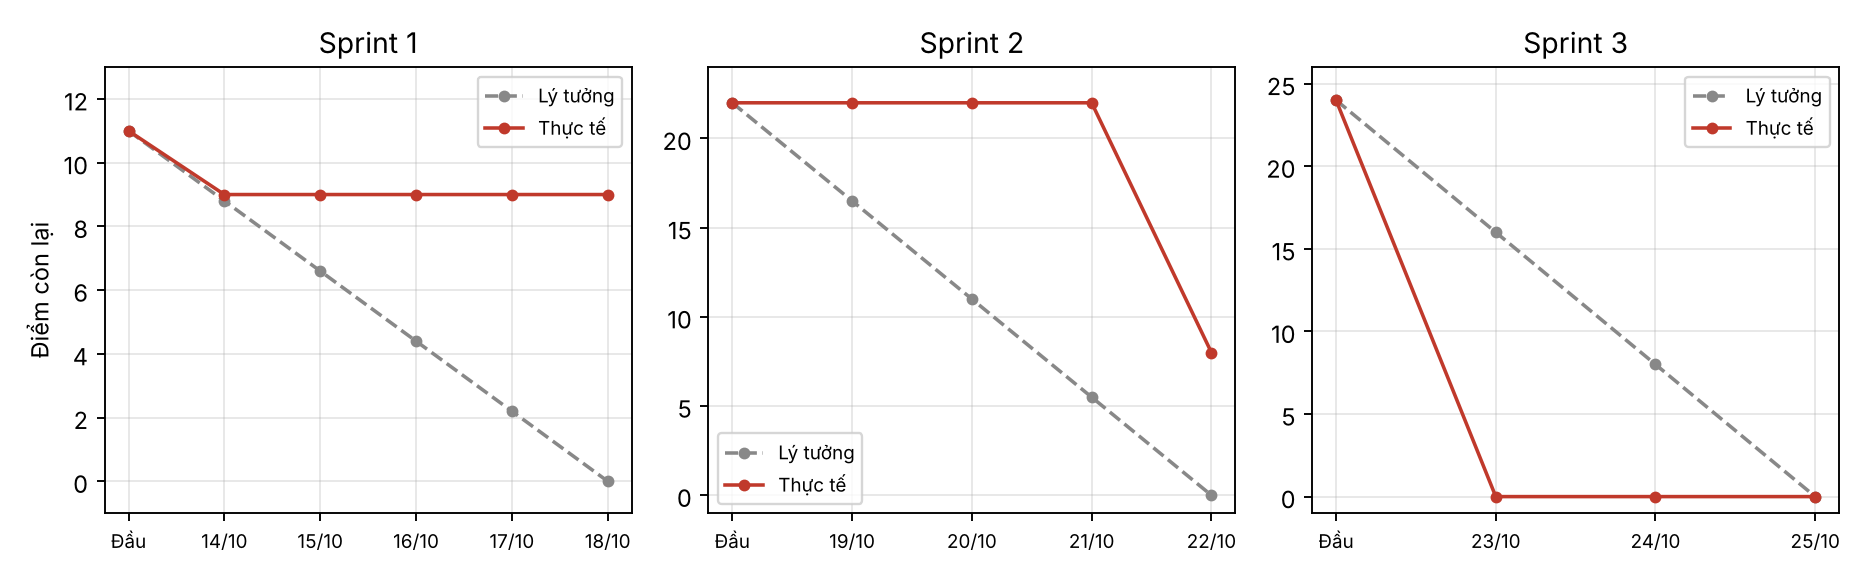
\includegraphics[width=\textwidth]{figures/burndown-3sprint.png}
\caption{\label{fig:burndown}Burndown ba Sprint (đường đứt: lý tưởng; đường liền: thực tế, tính theo ngày code lên Git). Điểm ước lượng: T1 = 2, T2--T5 = 3, T6--T8 = 5, T9 = 3, T10 = 8; điểm đầu Sprint là 11, 22, 24. Sprint 3 hoàn tất toàn bộ phần việc ngay ngày đầu (23/10).}
\end{figure}

\begin{center}
\begin{minipage}[t]{0.48\textwidth}\centering
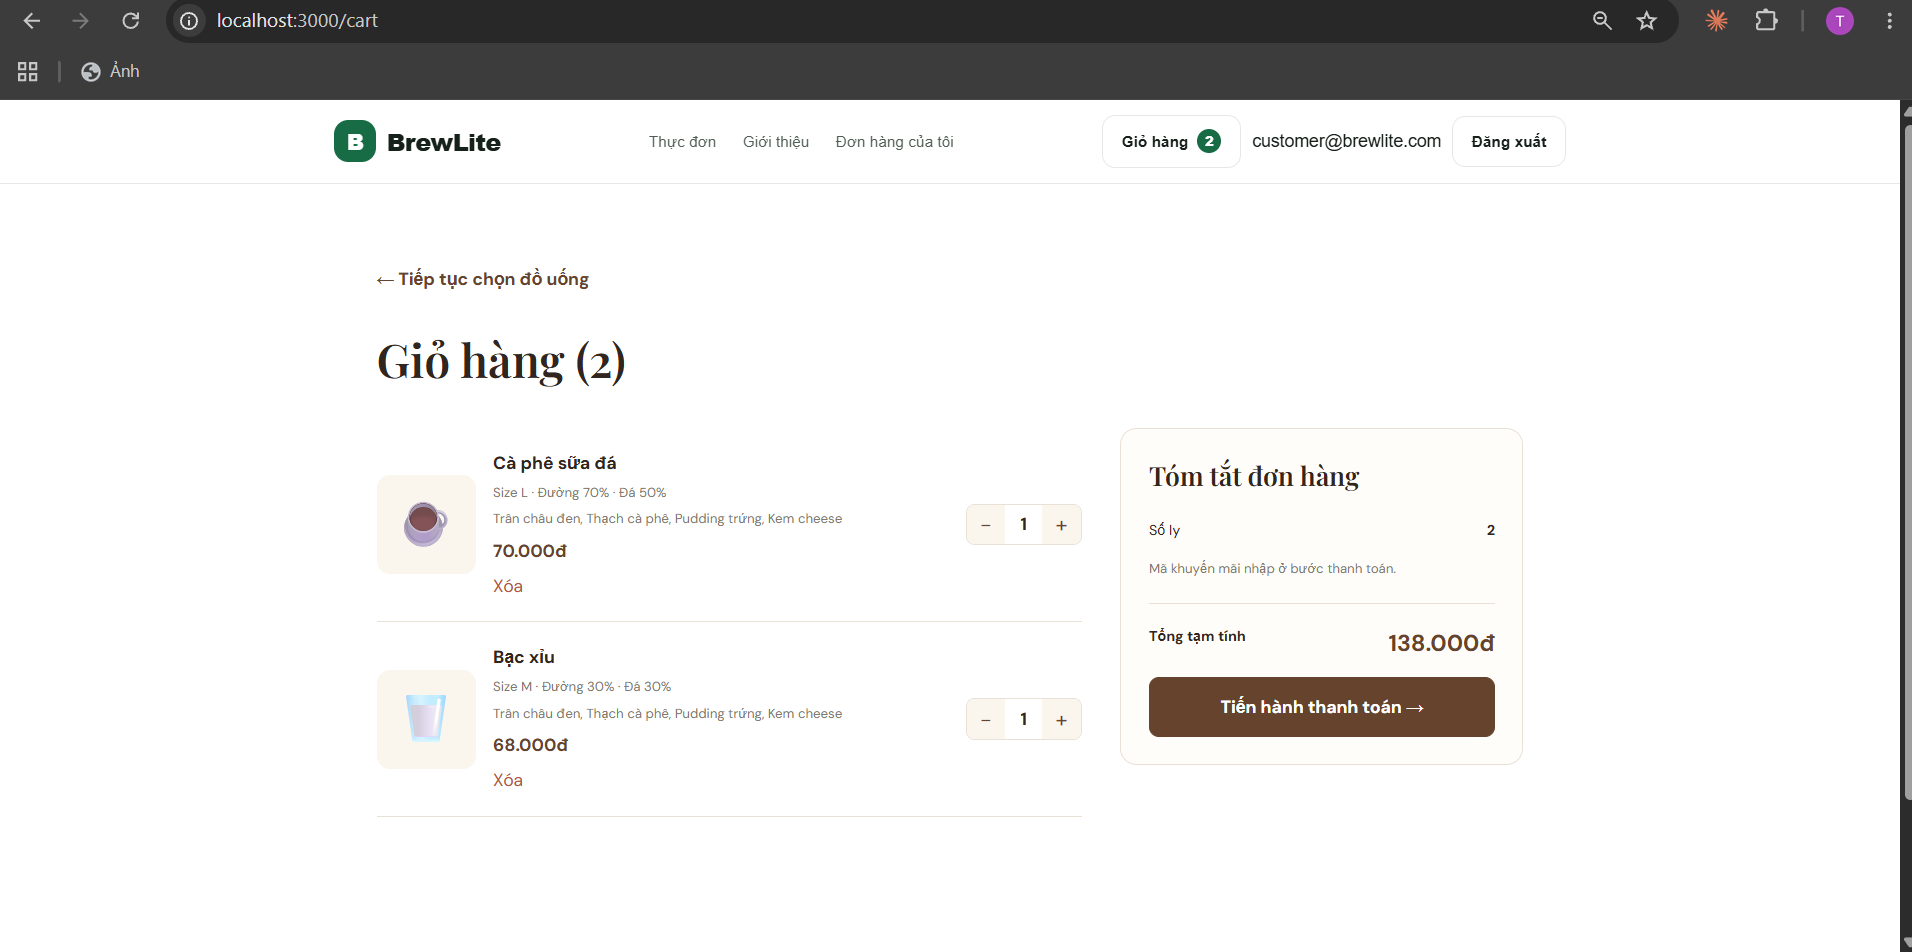
\includegraphics[width=\textwidth]{figures/ev03-gio-hang.png}
\captionof{figure}{Giỏ hàng (\texttt{/cart}): 2 món với size, mức đường/đá, topping; tạm tính 138.000đ}
\end{minipage}\hfill
\begin{minipage}[t]{0.48\textwidth}\centering
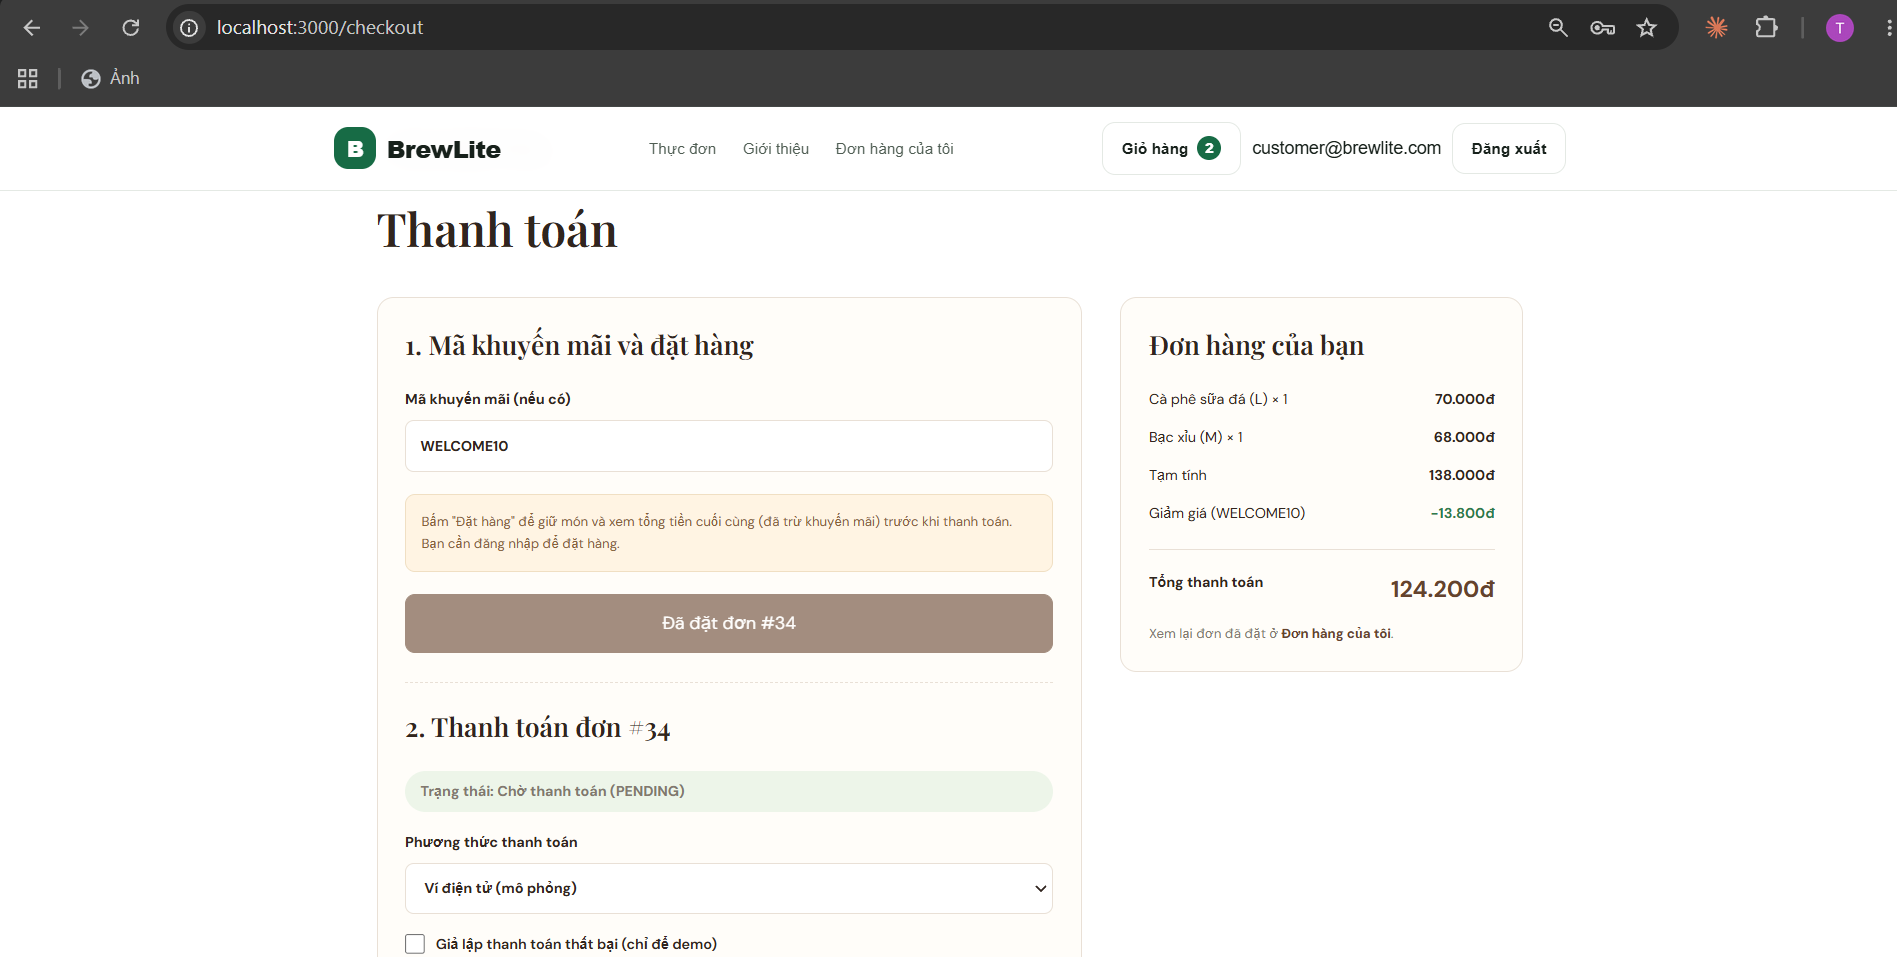
\includegraphics[width=\textwidth]{figures/ev04-thanh-toan-welcome10.png}
\captionof{figure}{Thanh toán (\texttt{/checkout}): đặt đơn \#34 với WELCOME10, máy chủ tính giảm 13.800đ, tổng 124.200đ}
\end{minipage}

\vspace{4mm}
\begin{minipage}[t]{0.48\textwidth}\centering
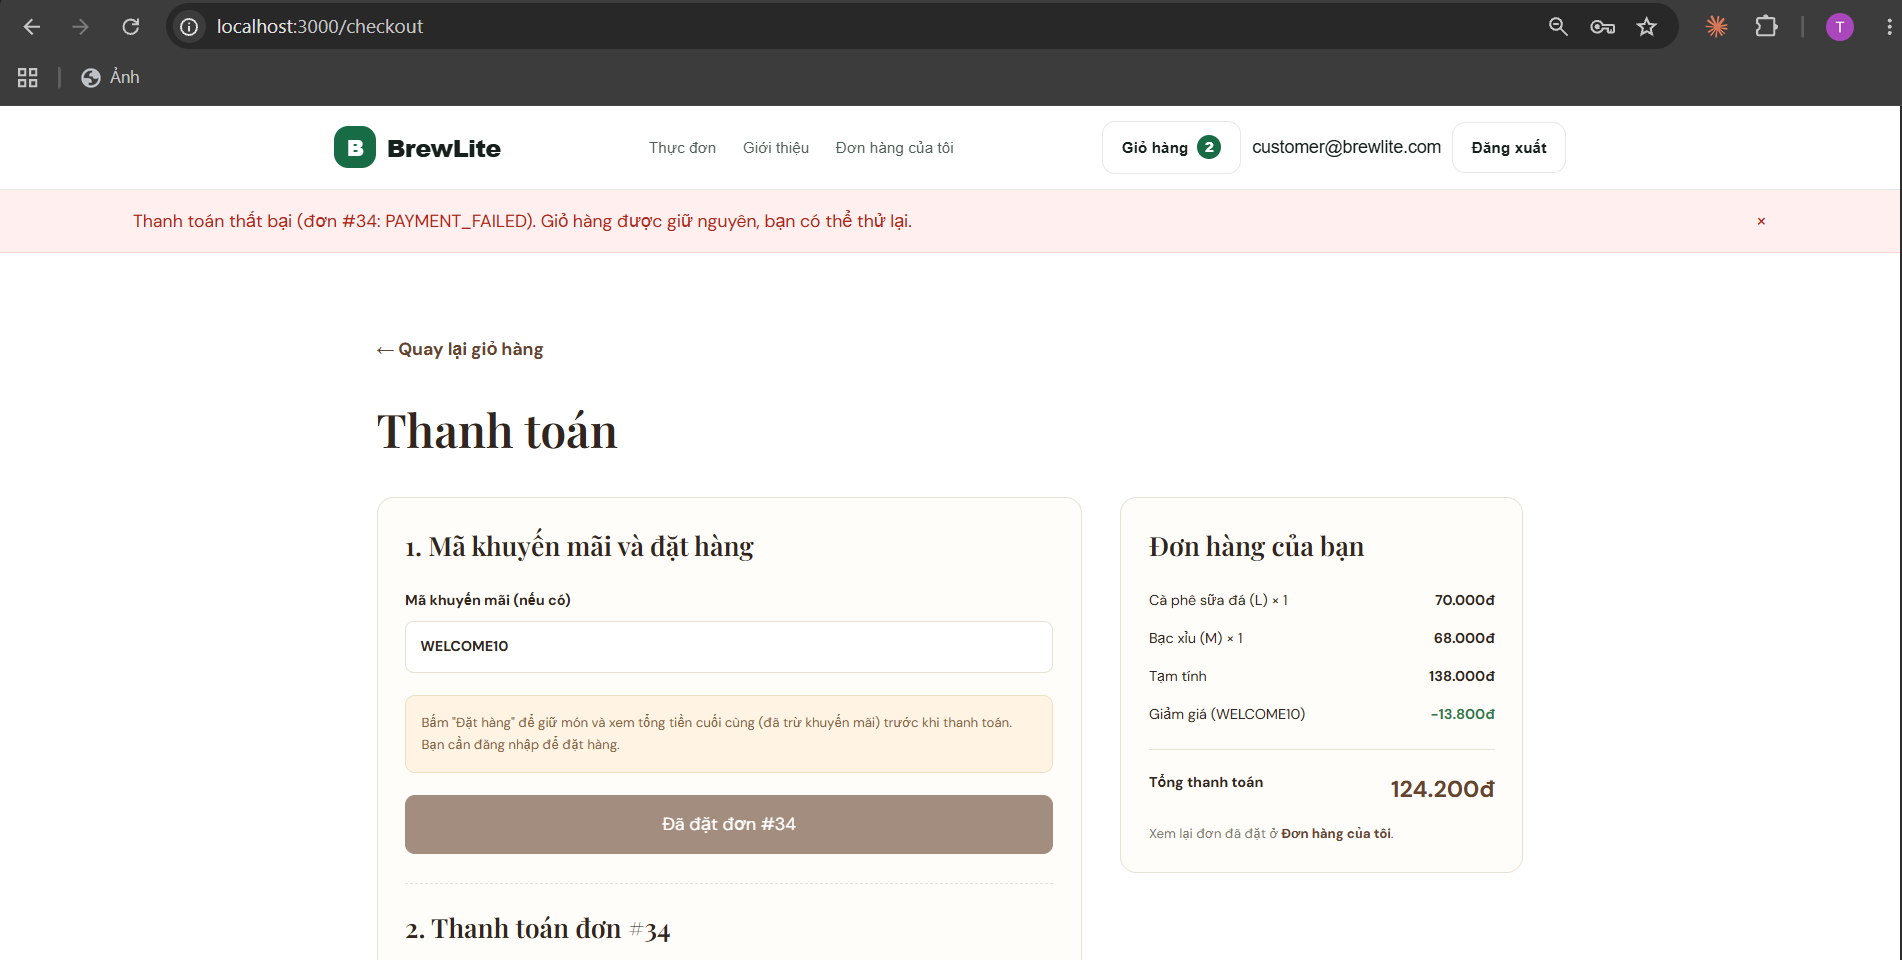
\includegraphics[width=\textwidth]{figures/ev09-thanh-toan-that-bai.png}
\captionof{figure}{Giả lập thanh toán lỗi: đơn \#34 PAYMENT\_FAILED, thông báo đỏ, giỏ hàng giữ nguyên}
\end{minipage}\hfill
\begin{minipage}[t]{0.48\textwidth}\centering
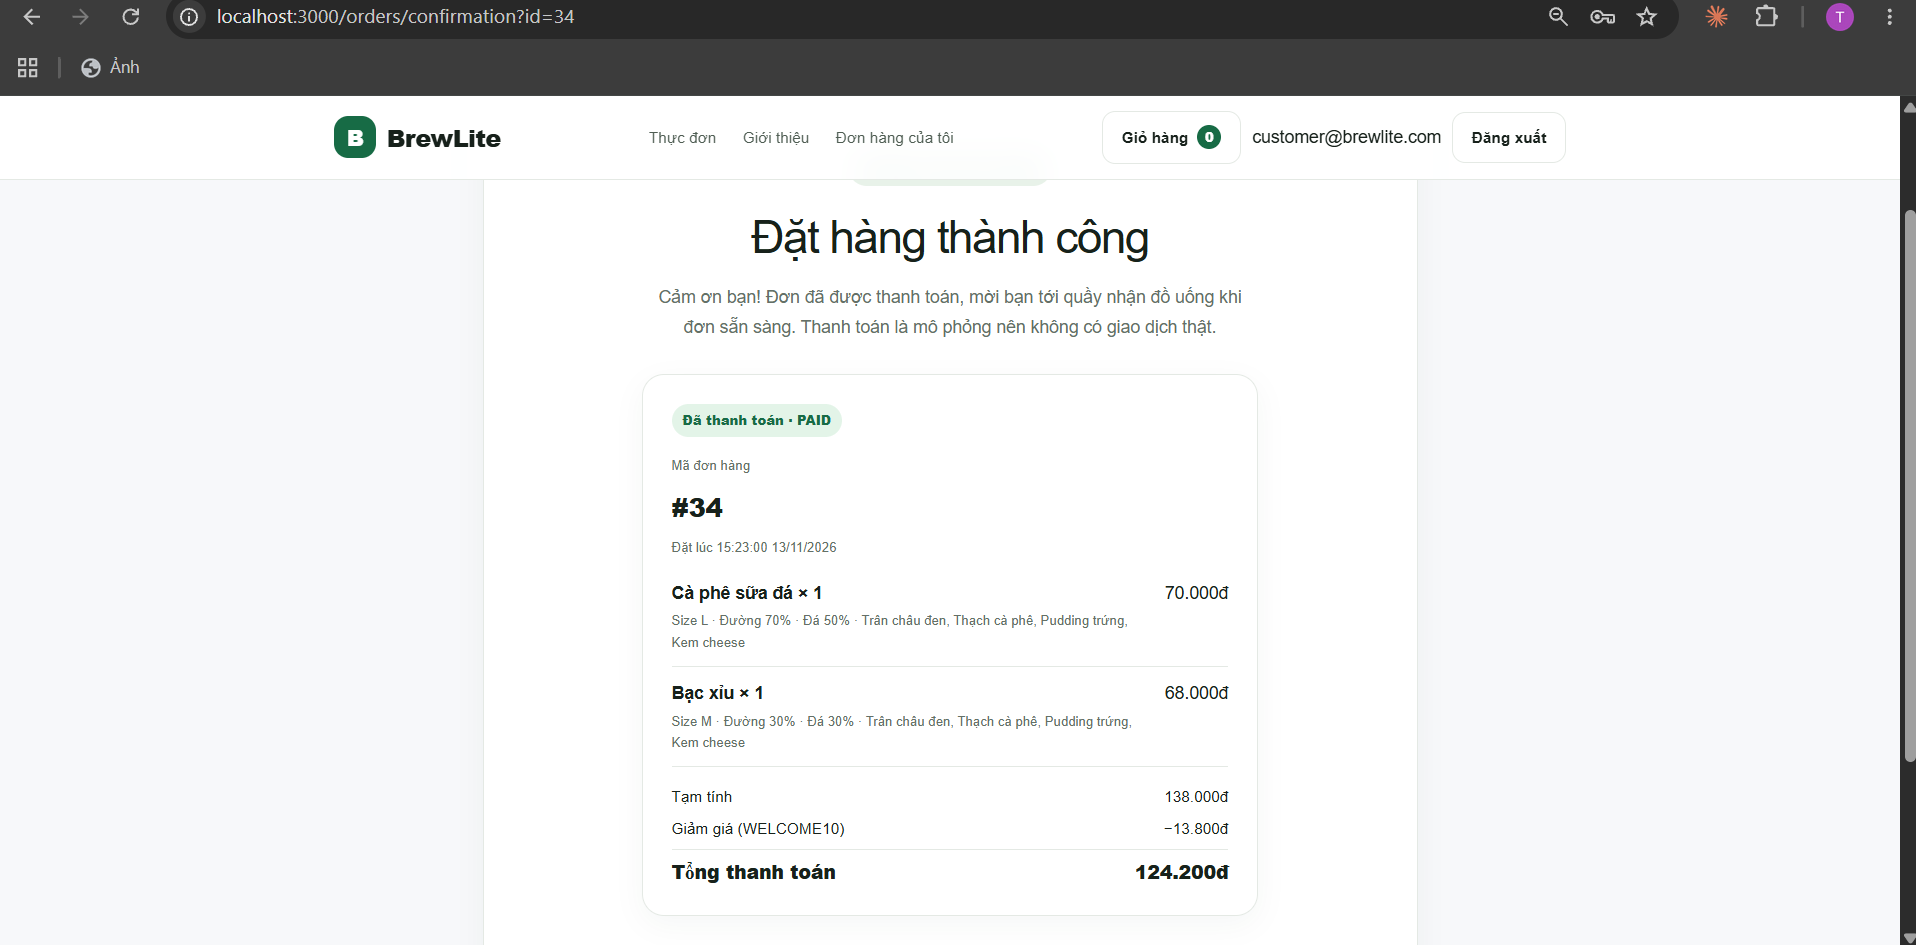
\includegraphics[width=\textwidth]{figures/ev10-xac-nhan-don-paid.png}
\captionof{figure}{Thử lại thành công: cùng đơn \#34 PAID; trang xác nhận có từng món, mức đường/đá, giảm giá}
\end{minipage}

\vspace{4mm}
\begin{minipage}[t]{0.48\textwidth}\centering
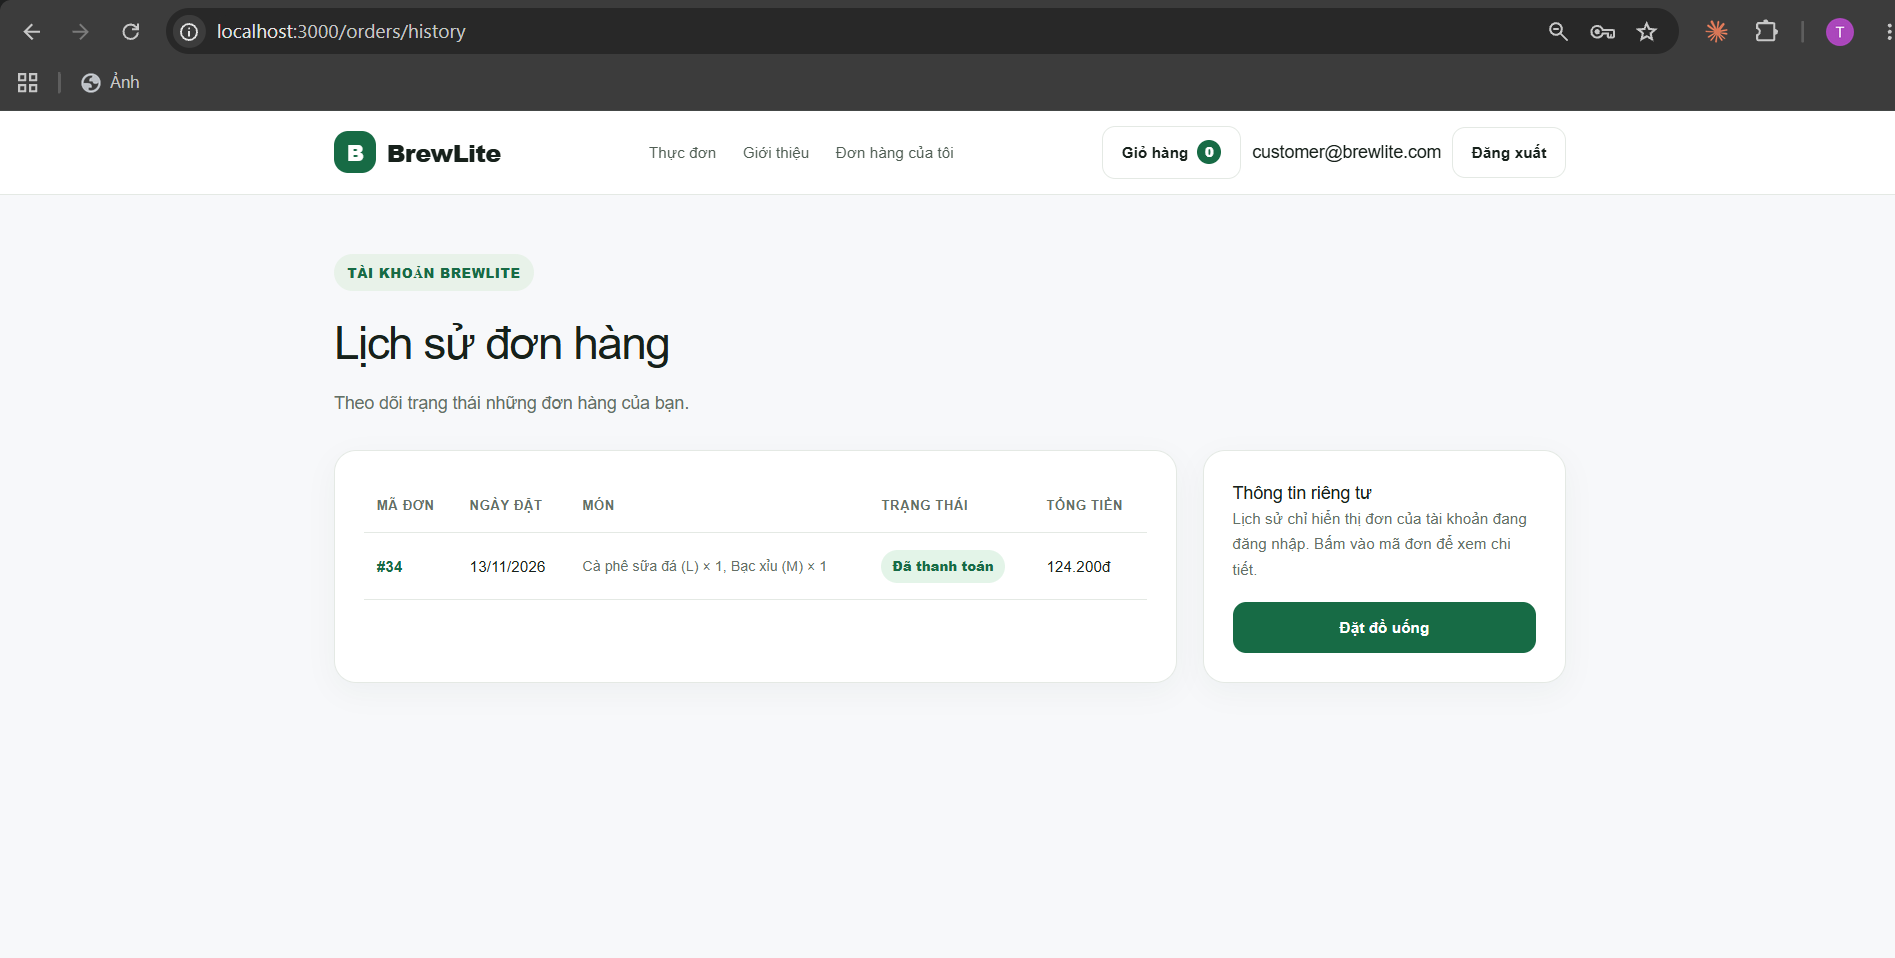
\includegraphics[width=\textwidth]{figures/ev06-lich-su.png}
\captionof{figure}{Lịch sử đơn: chỉ có đơn \#34, thử lại không tạo đơn trùng}
\end{minipage}\hfill
\begin{minipage}[t]{0.48\textwidth}\centering
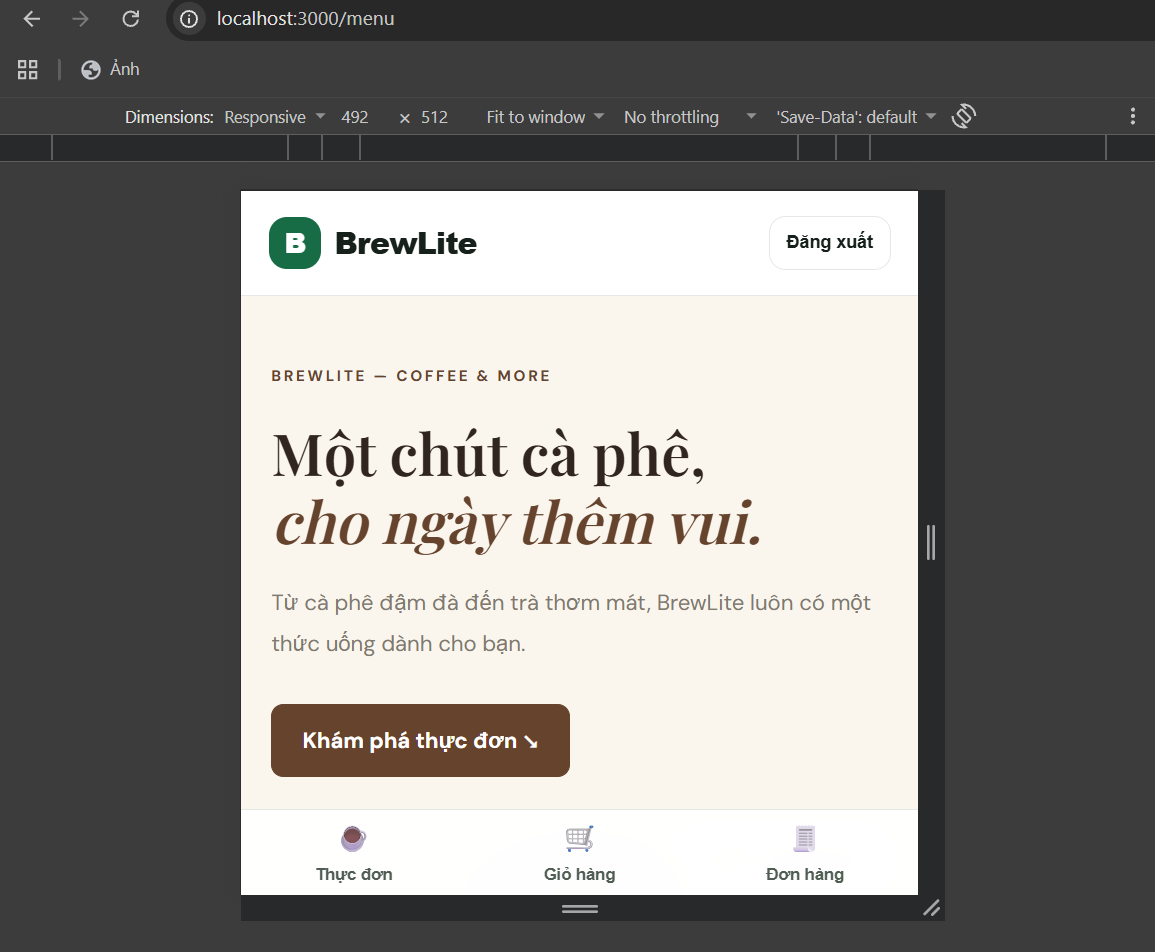
\includegraphics[width=0.75\textwidth]{figures/ev07-dien-thoai.png}
\captionof{figure}{Giao diện điện thoại: thanh tab Thực đơn, Giỏ hàng, Đơn hàng cố định ở đáy màn hình}
\end{minipage}
\end{center}

\begin{figure}[h!]
\centering
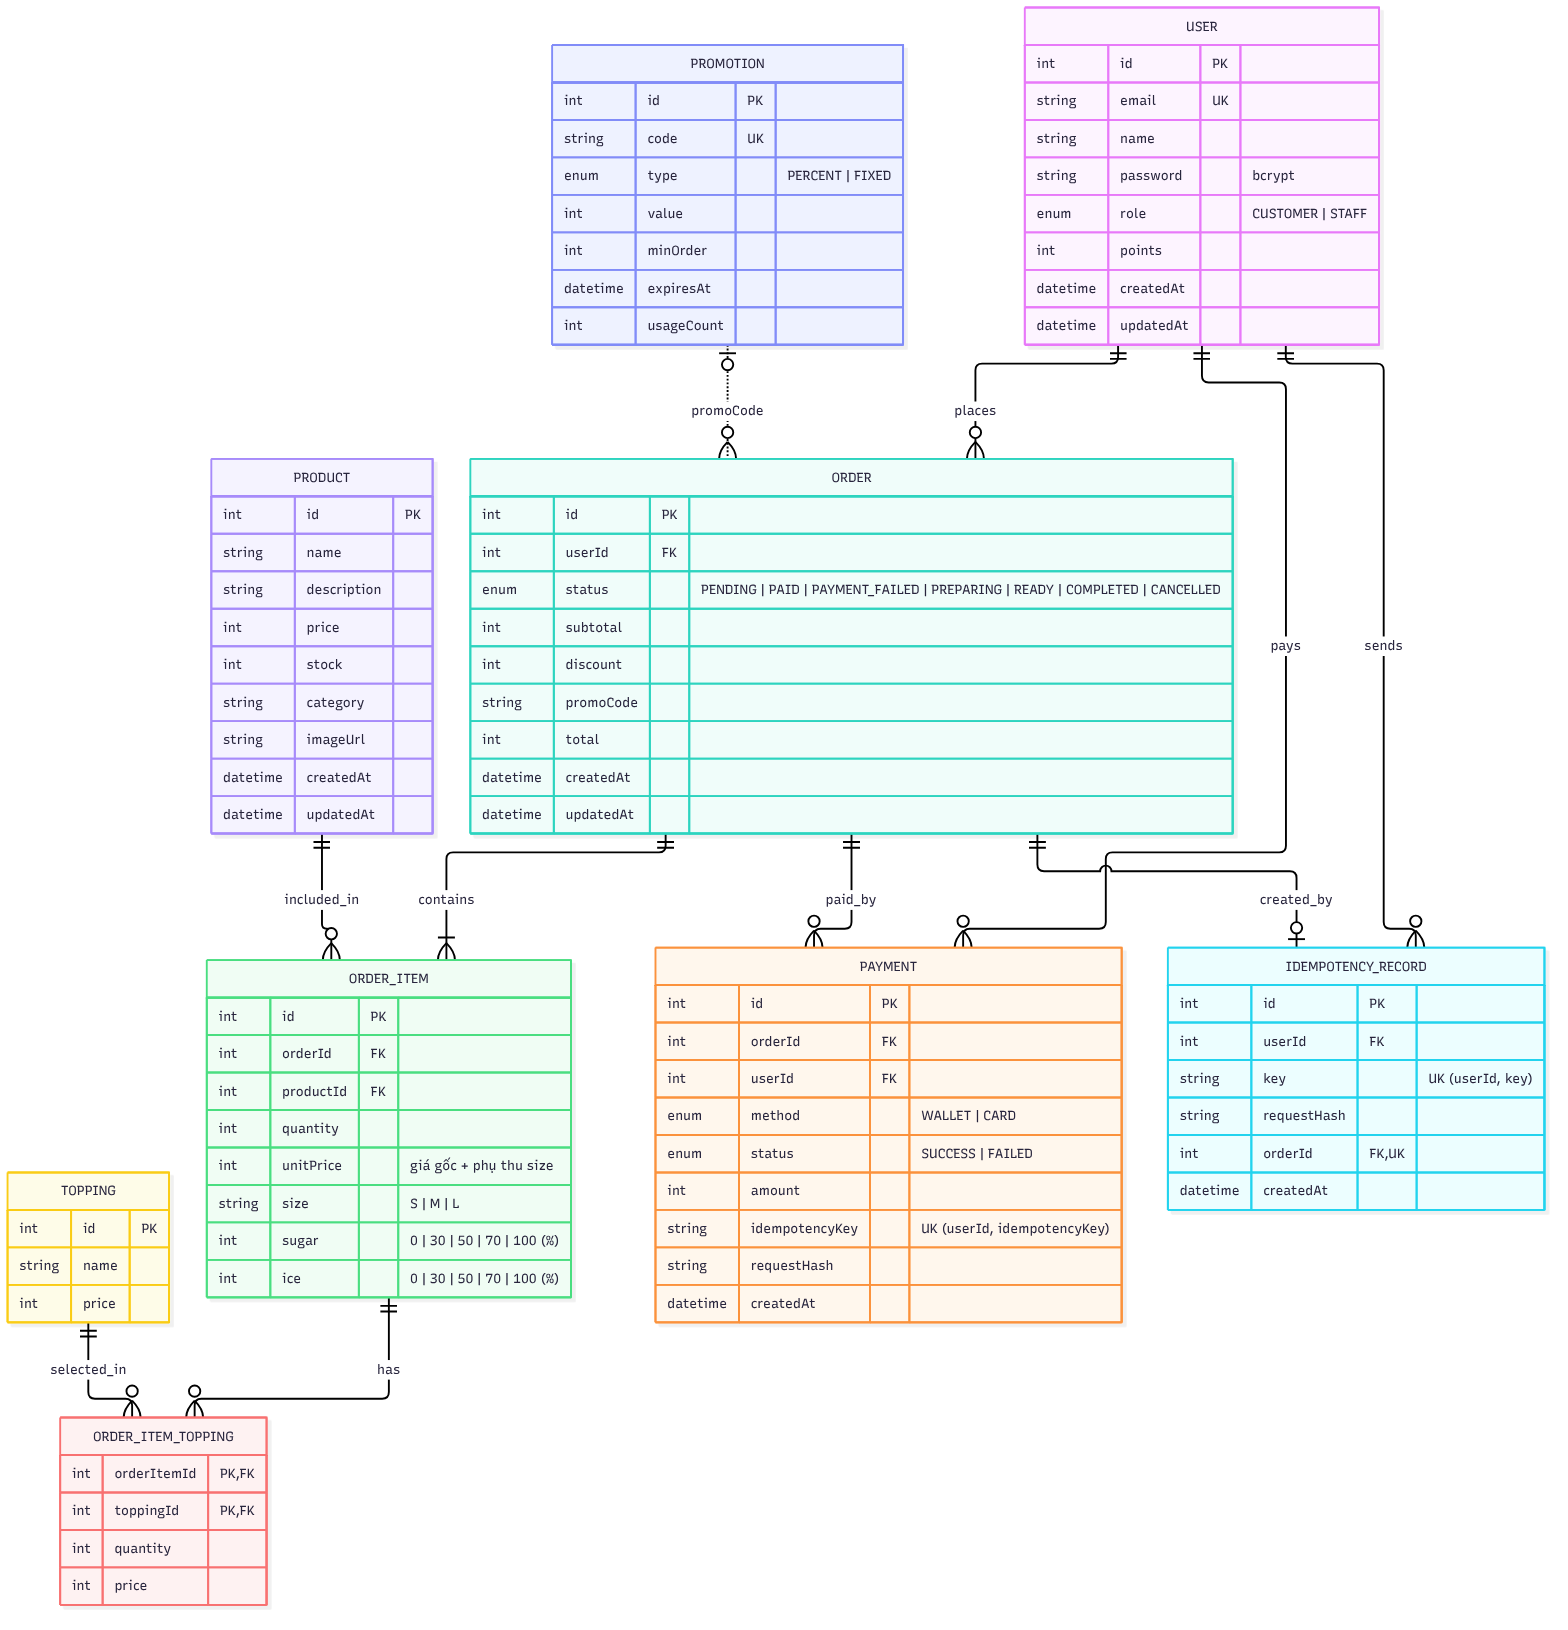
\includegraphics[width=0.85\textwidth]{figures/erd.png}
\caption{\label{fig:erd}Sơ đồ quan hệ dữ liệu (ERD), khớp \texttt{backend/prisma/schema.prisma}}
\end{figure}

\begin{figure}[h!]
\centering
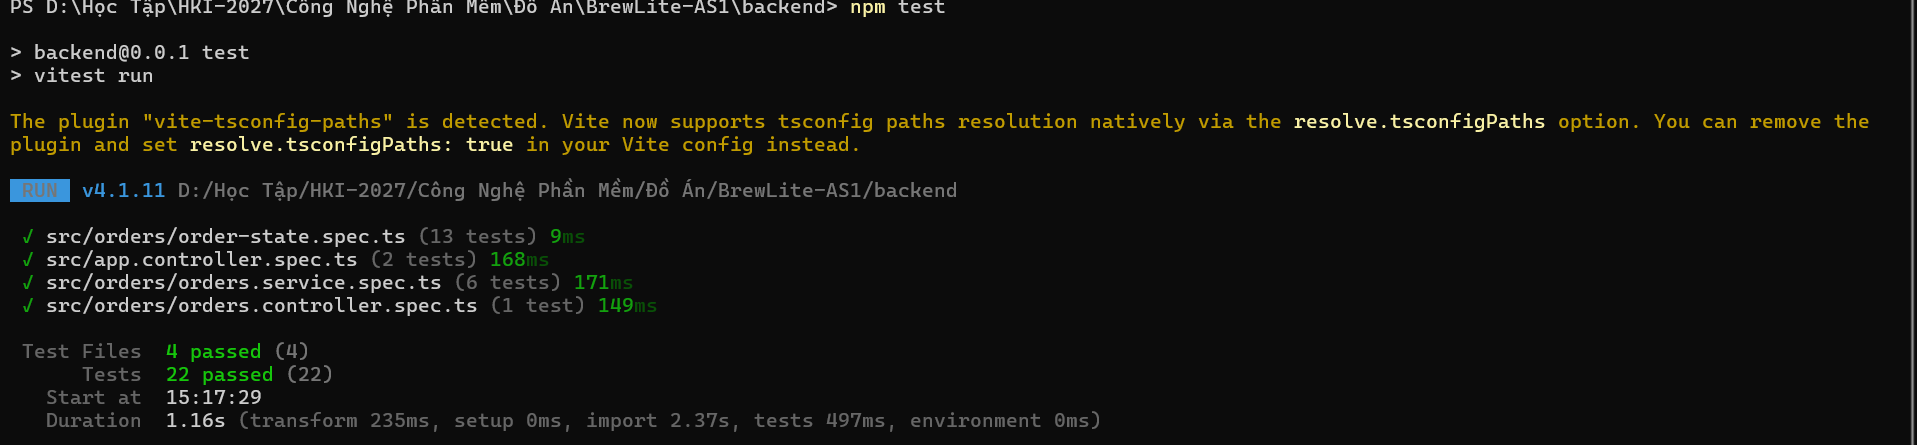
\includegraphics[width=\textwidth]{figures/ev11-unit-test-22.png}
\caption{\label{fig:testunit}Unit test (\texttt{npm test}): 4 tệp, 22/22 đạt}
\end{figure}

\begin{figure}[h!]
\centering
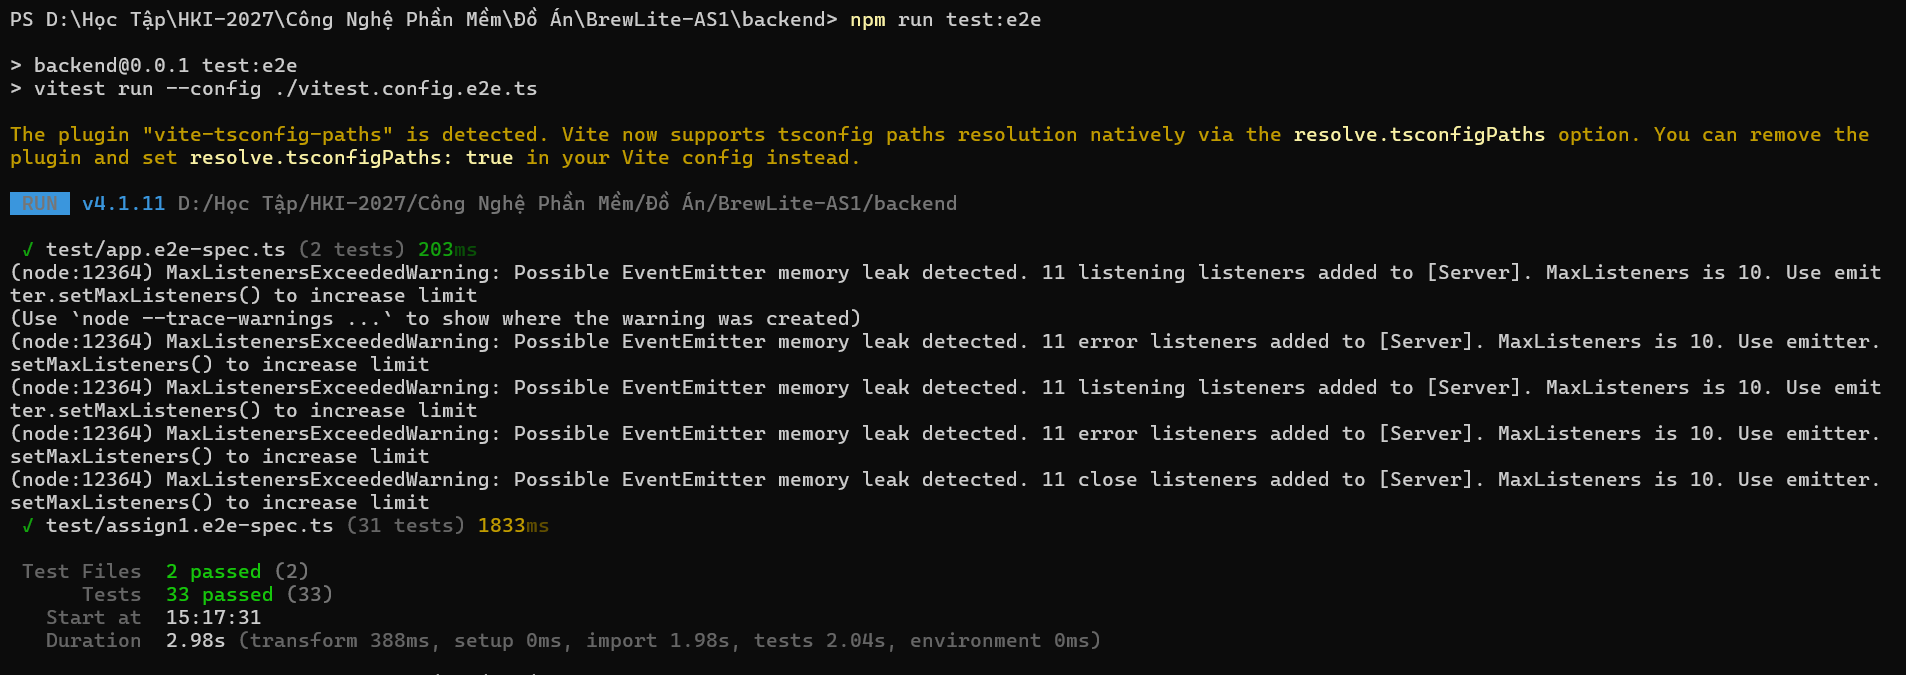
\includegraphics[width=\textwidth]{figures/ev12-e2e-test-33.png}
\caption{\label{fig:teste2e}Test tích hợp (\texttt{npm run test:e2e}, PostgreSQL thật), 2 tệp, 33/33 đạt}
\end{figure}

\end{document}
